%!TEX TS-program = lualatex
%!TEX encoding = UTF-8 Unicode

\documentclass[12pt, addpoints]{exam}
\usepackage{graphicx}
	\graphicspath{{/Users/goby/Pictures/teach/163/lab/}
	{img/}} % set of paths to search for images

\usepackage{geometry}
\geometry{letterpaper, left=1.5in, bottom=1in}                   
%\geometry{landscape}                % Activate for for rotated page geometry
\usepackage[parfill]{parskip}    % Activate to begin paragraphs with an empty line rather than an indent
\usepackage{amssymb, amsmath}
\usepackage{mathtools}
	\everymath{\displaystyle}

\usepackage{fontspec}
\setmainfont[Ligatures={TeX}, BoldFont={* Bold}, ItalicFont={* Italic}, BoldItalicFont={* BoldItalic}, Numbers={OldStyle}]{Linux Libertine O}
\setsansfont[Scale=MatchLowercase,Ligatures=TeX]{Linux Biolinum O}
\setmonofont[Scale=MatchLowercase]{Linux Libertine Mono O}
\usepackage{microtype}


% To define fonts for particular uses within a document. For example, 
% This sets the Libertine font to use tabular number format for tables.
 %\newfontfamily{\tablenumbers}[Numbers={Monospaced}]{Linux Libertine O}
% \newfontfamily{\libertinedisplay}{Linux Libertine Display O}

\usepackage{booktabs}
%\usepackage{multicol}

\usepackage{caption}
	\captionsetup{labelsep=period, justification=raggedright} % Removes colon following figure / table number.
	\captionsetup{singlelinecheck=off}
	\captionsetup[table]{skip=0pt}

\usepackage{tikz}
\tikzstyle{block} = [rectangle, draw, fill=white, rounded corners,
                 minimum size=2em]
\tikzstyle{branch} = [thick, draw]


\usepackage{longtable}
%\usepackage{siunitx}
\usepackage{array}
\newcolumntype{L}[1]{>{\raggedright\let\newline\\\arraybackslash\hspace{0pt}}p{#1}}
\newcolumntype{C}[1]{>{\centering\let\newline\\\arraybackslash\hspace{0pt}}p{#1}}
\newcolumntype{R}[1]{>{\raggedleft\let\newline\\\arraybackslash\hspace{0pt}}p{#1}}

\usepackage{enumitem}
%\usepackage{hyperref}
%\usepackage{placeins} %PRovides \FloatBarrier to flush all floats before a certain point.
%\usepackage{hanging}

\usepackage[sc]{titlesec}

%% Commands for Exam class
\renewcommand{\solutiontitle}{\noindent}
\unframedsolutions
\SolutionEmphasis{\bfseries}

\renewcommand{\questionshook}{%
	\setlength{\leftmargin}{-\leftskip}%
}

%Change \half command from 1/2 to .5
\renewcommand*\half{.5}

\pagestyle{headandfoot}
\firstpageheader{\textsc{bi}\,063 Evolution and Ecology}{}{\ifprintanswers\textbf{KEY}\else Name: \enspace \makebox[2.5in]{\hrulefill}\fi}
\runningheader{}{}{\footnotesize{pg. \thepage}}
\footer{}{}{}
\runningheadrule

\newcommand*\AnswerBox[2]{%
    \parbox[t][#1]{0.92\textwidth}{%
    \begin{solution}#2\end{solution}}
%    \vspace*{\stretch{1}}
}

\newenvironment{AnswerPage}[1]
    {\begin{minipage}[t][#1]{0.92\textwidth}%
    \begin{solution}}
    {\end{solution}\end{minipage}
    \vspace*{\stretch{1}}}

\newlength{\basespace}
\setlength{\basespace}{5\baselineskip}

%% To hide and show points
\newcommand{\hidepoints}{%
	\pointsinmargin\pointformat{}
}

\newcommand{\showpoints}{%
	\nopointsinmargin\pointformat{(\thepoints)}
}

\newcommand{\bumppoints}[1]{%
	\addtocounter{numpoints}{#1}
}

%
%\makeatletter
%\def\SetTotalwidth{\advance\linewidth by \@totalleftmargin
%\@totalleftmargin=0pt}
%\makeatother


%\printanswers


\begin{document}

\subsection*{D\textsc{na} similarities and phylogenetic trees (\numpoints\ points)}

This is what you should have come up with for the number of nucleotide differences among the different species.

\begin{longtable}[c]{@{}rR{0.25in}R{0.25in}R{0.25in}R{0.25in}R{0.25in}R{0.25in}@{}}
\toprule
& Y & C & B & R & F & A\tabularnewline[0.15in]
Y & 0 & 4 & 2 & 10 & 6 & 6\tabularnewline[0.15in]
C & & 0 & 4 & 10 & 6 & 6\tabularnewline[0.15in]
B & & & 0 & 10 & 6 & 6\tabularnewline[0.15in]
R & & & & 0 & 10 & 10\tabularnewline[0.15in]
F & & & &  & 0 & 2\tabularnewline[0.15in]
A & & &  &  &  & 0\tabularnewline[0.15in]
\bottomrule
\end{longtable}

\begin{questions}


\question[2]
Which species are the most similar? Why?

\AnswerBox{5\baselineskip}{%
 B and Y, and F and A. Both pairs differ by only two nucleotides, the fewest number of all pairs.
}

You can construct a phylogenetic tree  based on genetic similarity, following the steps
below. Try this on a piece of paper as you read along; you will do it for
real later (and possibly on an exam). 

\begin{enumerate}[leftmargin=*, label=\alph*.]

\item What species are the most similar? Put the letters at the top of the
chart. Put a dot below them opposite the number of nucleotide
differences between them. Draw lines connecting the two species to the
dot. Do this for each pair of very closely related species.

\item What species is most similar to one pair from part a? Put its letter
at the top and put a dot below it opposite the number of nucleotide
differences between it and either of the pair of species from part a.
Draw lines connecting the third species to the dot below the pair.

\item Repeat step b for each group of species, working from most similar to
least similar.

\end{enumerate}

The next several pages will walk you through this process. Be sure you understand each step so that you can do this on your own with different data.

\newpage

Set the diagram up like this, with a scale of nucleotide differences
down the side:

\begin{tikzpicture}[scale=0.8]

\draw (0,0) -- coordinate (y axis mid) (0,10);
    	%ticks
\foreach \y/\label in {0/10, 2/8, 4/6, 6/4, 8/2, 10/0}
	\draw (1pt,\y) -- (-3pt,\y) 
		node[anchor=east] {\label};                  
                 
\foreach \x/\species in {0/C, 2/B,4/F, 6/R, 8/Y, 10/A}
	\node [block] at (15,\x) (\species) {\species} ;
                 
\end{tikzpicture}

Plot two of the most similar, \textsc{b} and \textsc{y}. They show a difference of 2
nucleotides so connect the lines at 2. After you plot these, the
diagram should look like this.

\begin{tikzpicture}[scale=0.8]

\draw (0,0) -- coordinate (y axis mid) (0,10);
    	%ticks
\foreach \y/\label in {0/10, 2/8, 4/6, 6/4, 8/2, 10/0}
	\draw (1pt,\y) -- (-3pt,\y) 
		node[anchor=east] {\label};                  

\node [block] at (2,10.5) (b) {B};
\node [block] at (4,10.5) (y) {Y};
\path[branch] (b.south) -- (3,8);
\path[branch] (y.south) -- (3,8);
                 
\foreach \x/\species in {0/C, 4/F, 6/R, 10/A}
	\node [block] at (15,\x)  {\species} ;
                 
\end{tikzpicture}

\newpage

Now add \textsc{y}, which is the next lowest number (and therefore next most similar).  C is different from \textsc{y} by 4.  It is also 4 from \textsc{b}, so this fits.  It now looks like this.

\begin{tikzpicture}[scale=0.8]

\draw (0,0) -- coordinate (y axis mid) (0,10);
    	%ticks
\foreach \y/\label in {0/10, 2/8, 4/6, 6/4, 8/2, 10/0}
	\draw (1pt,\y) -- (-3pt,\y) 
		node[anchor=east] {\label};                  

\node [block] at (2,10.5) (b) {B};
\node [block] at (4,10.5) (y) {Y};
\node [block] at (6,10.5) (c) {C};

\node (by) at (3,8){};
\node (byc) at (5,6){};

\path [branch] (b.south) -- (by.center); 
\path [branch] (y.south) -- (by.center);
\path [branch] (c.south) -- (byc.center);
\path [branch] (by.center) -- (byc.center);
                 
\foreach \x/\species in {4/F, 6/R, 10/A}
	\node [block] at (15,\x)  {\species} ;
                 
\end{tikzpicture}

F and \textsc{a} are also only separated by 2 so connect them like \textsc{b} and \textsc{y}.

\begin{tikzpicture}[scale=0.8]

\draw (0,0) -- coordinate (y axis mid) (0,10);
    	%ticks
\foreach \y/\label in {0/10, 2/8, 4/6, 6/4, 8/2, 10/0}
	\draw (1pt,\y) -- (-3pt,\y) 
		node[anchor=east] {\label};                  

\node [block] at (2,10.5) (b) {B};
\node [block] at (4,10.5) (y) {Y};
\node [block] at (6,10.5) (c) {C};
\node [block] at (8,10.5) (f) {F};
\node [block] at (10,10.5) (a) {A};

\node (by) at (3,8){};
\node (byc) at (5,6){};
\node (fa) at (9,8){};

\path [branch] (b.south) -- (by.center); 
\path [branch] (y.south) -- (by.center);
\path [branch] (c.south) -- (byc.center);
\path [branch] (by.center) -- (byc.center);
\path [branch] (f.south) -- (fa.center);
\path [branch] (a.south) -- (fa.center);
                 
\foreach \x/\species in {6/R}
	\node [block] at (15,\x)  {\species} ;
                 
\end{tikzpicture}

\newpage

Now connect the \textsc{f} and \textsc{a} pair to \textsc{b}, \textsc{y}, and \textsc{c}.  F is 6 from \textsc{b}, \textsc{y}, and \textsc{c}.  A is also 6 from each of those three so they should all connect at 6.  It looks like this.

\begin{tikzpicture}[scale=0.8]

\draw (0,0) -- coordinate (y axis mid) (0,10);
    	%ticks
\foreach \y/\label in {0/10, 2/8, 4/6, 6/4, 8/2, 10/0}
	\draw (1pt,\y) -- (-3pt,\y) 
		node[anchor=east] {\label};                  

\node [block] at (2,10.5) (b) {B};
\node [block] at (4,10.5) (y) {Y};
\node [block] at (6,10.5) (c) {C};
\node [block] at (8,10.5) (f) {F};
\node [block] at (10,10.5) (a) {A};

\node (by) at (3,8){};
\node (byc) at (5,6){};
\node (fa) at (9,8){};
\node (bycfa) at (7,4){};

\path [branch] (b.south) -- (by.center); 
\path [branch] (y.south) -- (by.center);
\path [branch] (c.south) -- (byc.center);
\path [branch] (by.center) -- (byc.center);
\path [branch] (f.south) -- (fa.center);
\path [branch] (a.south) -- (fa.center);
\path [branch] (fa.center) -- (bycfa.center);
\path [branch] (byc.center) -- (bycfa.center);

\foreach \x/\species in {6/R}
	\node [block] at (15,\x)  {\species} ;
                 
\end{tikzpicture}

Finally, connect \textsc{r} to the rest.  It is 10 from all of the other species so the connection is back at 10.

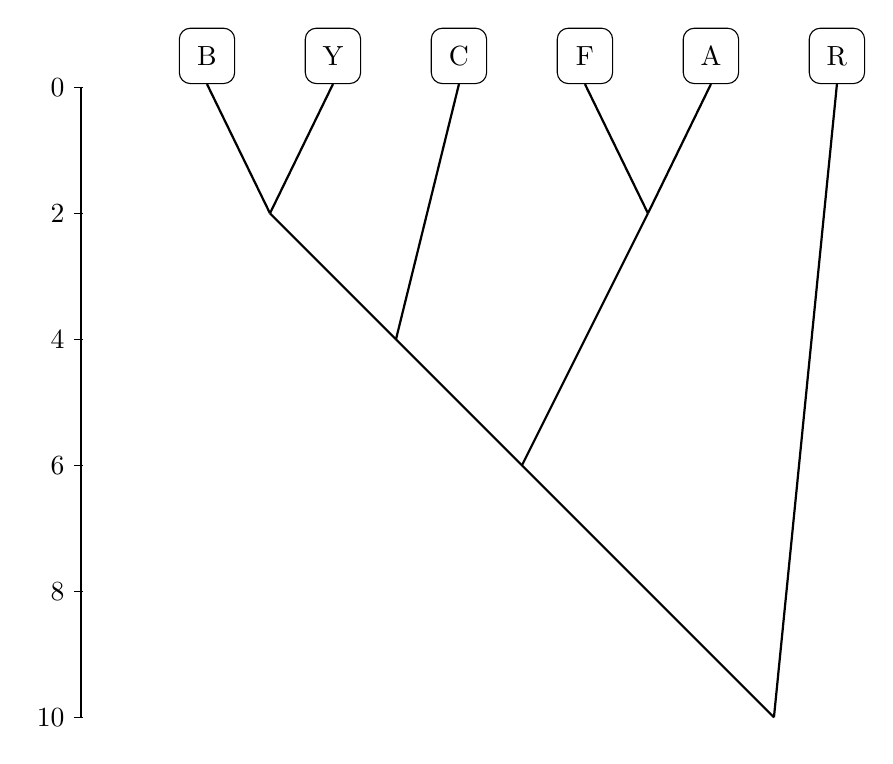
\begin{tikzpicture}[scale=0.8]

\draw (0,0) -- coordinate (y axis mid) (0,10);
    	%ticks
\foreach \y/\label in {0/10, 2/8, 4/6, 6/4, 8/2, 10/0}
	\draw (1pt,\y) -- (-3pt,\y) 
		node[anchor=east] {\label};                  

\node [block] at (2,10.5) (b) {B};
\node [block] at (4,10.5) (y) {Y};
\node [block] at (6,10.5) (c) {C};
\node [block] at (8,10.5) (f) {F};
\node [block] at (10,10.5) (a) {A};
\node [block] at (12,10.5) (r) {R};

\node (by) at (3,8){};
\node (byc) at (5,6){};
\node (fa) at (9,8){};
\node (bycfa) at (7,4){};
\node (all) at (11,0){};

\path [branch] (b.south) -- (by.center); 
\path [branch] (y.south) -- (by.center);
\path [branch] (c.south) -- (byc.center);
\path [branch] (by.center) -- (byc.center);
\path [branch] (f.south) -- (fa.center);
\path [branch] (a.south) -- (fa.center);
\path [branch] (fa.center) -- (bycfa.center);
\path [branch] (byc.center) -- (bycfa.center);
\path [branch] (bycfa.center) -- (all.center);
\path [branch] (r.south) -- (all.center);

\end{tikzpicture}

To check your work, go back to the table.  Check every number.  They should all fit.

Now you have a diagram that shows the number of nucleotide differences between any two species.  If you want to know how different, say, the blue-throated garbler (\textsc{b}) and the field twitterer (\textsc{f}) are,  just follow the lines down from both of them until you come to the spot where they join.  Then look over to the side and see how many nucleotide differences there are at that point—it will be 6, which is what was in the table. The diagram is a phylogenetic tree based on genetic differences.  

The genetic differences can be converted to time since the species last shared a common ancestor. Many studies have shown that mutations occur at a relatively constant rate over time. A regular rate of mutation is called a \textit{molecular clock.} If you know the mutation rate, then you can estimate when two species last shared an ancestor. For example, if mutations occur at a rate of about 2\% per million years, then two species that differ by 6\% split from their common ancestor about 3 million years ago. You will learn more about molecular clocks in lecture. 

Here are the data and bird names again:

\begin{longtable}[c]{@{}ll@{}}
\toprule
Yellow-throated Garbler \textsc{(y)} & {\ttfamily CTAGC AAGTA CTACT TAGGA}\tabularnewline
California Garbler \textsc{(c)} & {\ttfamily CTGGC AAGTA CTTCT TAAGG}\tabularnewline
Blue-throated Garbler \textsc{(b)} & {\ttfamily CTAGC AACTA CTACT TAAGA}\tabularnewline
Red-footed Chump \textsc{(r)} & {\ttfamily AGGCC ATGGA CGACT ACAGA}\tabularnewline
Field Twitterer \textsc{(f)} & {\ttfamily CTGGA AAGGC CTAGT TAAGA}\tabularnewline
Alfredo's Twitterer \textsc{(a)} & {\ttfamily CTGGA AAGGA CTAGG TAAGA}\tabularnewline
\bottomrule
\end{longtable}

\question[3]
Using your completed diagram, you can divide these
birds into groups of close relatives. One way would be to group them as
garblers, twitterers, and chumps. Why is this a reasonable way
to group them, based on your comparison of their \textsc{dna}?

\AnswerBox{3\baselineskip}{%
Because each group shares the fewest number of nucleotide differences.
}

\question[1]
How many nucleotides are different between the field
twitterer and the yellow-throated garbler?

\AnswerBox{0.5\baselineskip}{6}

\question[1]
Between the Alfredo's twitterer and the California garbler?

\AnswerBox{0.5\baselineskip}{6}

\question[3]
Why are these the same? \emph{Hint:} They should only be the same if
the molecular clock assumption is correct.

\AnswerBox{1\baselineskip}{%
They must have all shared a common ancestor at the same point in time in the past. They diverged from their common ancestor at the same time.
}

\newpage

\subsubsection*{Phylogeny of the primates}

You can compare genetic similarity of organisms with other methods, too. One 
way to determine similarity is a technique called \textsc{dna-dna} hybridization.
Strands of \textsc{dna}  from two different organisms 
are allowed to join by complementary base
pairing. The more similar their sequences are, the more bonding there
will be between the two strands. These hybrid double-stranded \textsc{dna} molecules are
then heated to separate them. The more tightly bonded the strands are, the
higher the temperature required to separate them. The temperature at
which the two strands from different species separate is compared to the
temperature at which two strands from the same species separate. The more similar
the species are, the less temperature difference there will be. 

In a previous study, \textsc{dna-dna} hybridization was used to compare the total \textsc{dna} 
of several primates. It turned out
that 1°\textsc{c} temperature difference corresponds to about 1\% difference in
\textsc{dna} sequence. The
table below gives the genetic difference (distance) between primate species, based on the temperatures required to separate
same-species versus different-species hybrid molecules.  The presented data are average temperature differences from several trials.

\vspace{\baselineskip}

\begin{longtable}[l]{@{}L{0.11\textwidth}C{0.11\textwidth}C{0.11\textwidth}C{0.11\textwidth}C{0.11\textwidth}C{0.11\textwidth}C{0.11\textwidth}C{0.11\textwidth}@{}}
\caption{Distance values among primates determined from \textsc{dna-dna}
hybridization.}\\
\toprule
 & H	& PC 	& CC & G & O & WHG \\
 \midrule
PC	& 1.64	&&&&&\\ 
CC	& 1.64	& 0.73 &&&&\\ 
G	& 2.32	& 2.32 & 2.32 &&&\\  
O	& 3.57	& 3.57 & 3.57 & 3.57 &&\\ 
WHG	& 4.79	& 4.79 & 4.79 & 4.79 & 4.79 &\\ 
CM & 7.21 & 7.21 & 7.21 & 7.21 & 7.21 & 7.21 \\
\bottomrule
\multicolumn{7}{@{}L{\textwidth}@{}}{\textsc{h} = human, \textsc{pc} = pygmy chimpanzee, 
\textsc{cc} = common chimpanzee, \textsc{g} = gorilla, \textsc{o} = orangutan,
\textsc{whg} = white-handed gibbon, \textsc{cm} = cerpithecoid monkey (macaque).}\\
\end{longtable}

You can use these data just as you did with the bird data to create a
phylogenetic tree showing relationships between these primates. You can review the previous
where you did this with bird \textsc{dna} to be confident of the technique.

\question[5]
Draw your tree of primates in the space provided for you on the next page.

\newpage

Write the seven organisms in a row across the top above the 0 line.  
The scale on the left is percent \textsc{dna} difference.  Do not 
worry if you cannot figure out exactly where to put 2.79 or whatever; 
put it in approximately the right spot. You can use the letter codes for the
primates: \textsc{h} = human, \textsc{pc} = pygmy chimpanzee, 
\textsc{cc} = common chimpanzee, \textsc{g} = gorilla, \textsc{o} = orangutan,
\textsc{whg} = white-handed gibbon, \textsc{cm} = cerpithecoid monkey.

\vspace*{3\baselineskip}

\setlength{\parindent}{-0.9cm}

\begin{tikzpicture}

\draw (0,0) [xscale=1.3] [thick] -- coordinate (x axis mid) (10.8,0);

\draw (0,0) [yscale=1.5,thick] -- coordinate (y axis mid) (0, 8);

\foreach \y / \label in {0/8,1/7, 2/6, 3/5, 4/4, 5/3, 6/2, 7/1,8/0}
	\draw [yscale=1.5] (1pt, \y) -- (-4pt,\y)
		node[anchor=east] {\label};

\node [rotate=90, above=0.8cm] at (y axis mid) {Genetic distance};

\ifprintanswers

\node [block] at (1,12.5) (cc) {CC};
\node [block] at (3,12.5) (pc) {PC};
\node [block] at (5,12.5) (h) {H};
\node [block] at (7,12.5) (g) {G};
\node [block] at (9,12.5) (o) {O};
\node [block] at (11,12.5) (whg) {WHG};
\node [block] at (13,12.5) (cm) {CM};

\node (ccpc) at (2,11){};
\node (ch) at (4,9.5){};
\node (chg) at (6,8.4){};
\node (chgo) at (8,6.7){};
\node (chgog) at (10, 5){};
\node (all) at (12,1){};

\path [branch] (cc.south) -- (ccpc.center); 
\path [branch] (pc.south) -- (ccpc.center);
\path [branch] (h.south) -- (ch.center);
\path [branch] (ccpc.center) -- (ch.center);
\path [branch] (g.south) -- (chg.center);
\path [branch] (ch.center) -- (chg.center);
\path [branch] (o.south) -- (chgo.center);
\path [branch] (chg.center) -- (chgo.center);
\path [branch] (chgo.center) -- (chgog.center);
\path [branch] (whg.south) -- (chgog.center);
\path [branch] (chgog.center) -- (all.center);
\path [branch] (cm.south) -- (all.center);


\node [right] at (1,1){H can be leftmost, with chimps inside of that.};
\fi


\end{tikzpicture}

\end{questions}

\end{document}  